\documentclass{article}
\usepackage[utf8]{inputenc}
\usepackage[spanish]{babel}
\usepackage{listings}
\usepackage{graphicx}
\graphicspath{ {images/} }
\usepackage{cite}

\begin{document}

\begin{titlepage}
    \begin{center}
        \vspace*{1cm}
            
        \Huge
        \textbf{Informa2 S.A.S}
            
        \vspace{0.5cm}
        \LARGE
        Parcial 2 - Análisis y diseño 
            
        \vspace{1.5cm}
            
        \textbf{Carolina Jimenez Restrepo}
            
        \vfill
            
        \vspace{0.8cm}
            
        \Large
        Despartamento de Ingeniería Electrónica y Telecomunicaciones\\
        Universidad de Antioquia\\
        Medellín\\
        Septiembre de 2021
            
    \end{center}
\end{titlepage}

\tableofcontents
\newpage
\section{Sección introductoria}\label{intro}
Análisis y diseño del segundo parcial, presentar una imagen en matriz de LEDs RGB 

\subsection{Análisis y diseño}
\
Luego de leer y analizar el desafío propuesto para el parcial 2 se tiene una idea de cómo dar solución a este, lo primero que se debe tener en cuenta son los requerimientos del desafío el cual nos pide ajustar las dimensiones de una imagen para proyectarlas en una matriz de LEDs RGB, así mismo como crear la matriz y hacer el montaje de la parte eléctrica que permitirá su funcionamiento.\\
Para la parte de ajustar las dimensiones de la imagen que sería submuestreo (disminución de la resolución) y sobremuestreo (aumento de la resolución) se creara un código que realice estos procesos, sin ayuda de librerías como lo indican las instrucciones del desafío, el siguiente paso es guardar una nueva imagen con estas nuevas dimensiones para luego obtener los datos correspondientes a esta imagen y escribirlos en un archivo txt el cual será utilizado en la plataforma tinkercad para la generación de una matriz de colores que junto con otras líneas de código nos permitirán ver la imagen proyectada en la matriz de LEDs RGB.\\
Para el montaje de la matriz LEDs RGB se utilizan 10 tiras de LEDs RGB lo cual nos genera una matriz 10x10 un Arduino y una fuente de voltaje que nos permitirán alimentar la matriz.\\
Para el desarrollo del algoritmo se crea en el entorno Qt una clase que contiene métodos los cuales van a permitir realizar el proceso de escalado de imagen (submuestreo y sobremuestreo), guardar la nueva imagen y escribir la información en un txt, comprobar si lo cargado es una imagen. La clase y los métodos mencionados pueden variar a medida que se va desarrollando el proyecto.


\section{Inclusión de imágenes} \label{imagenes}

En la Figura (\ref{fig:Matriz leds.png}), se presenta la matriz de LEDs con la que se trabajara, esta matriz esta dispuesta a cambios segun lo requiera el avance del desafio 

\begin{figure}[h]
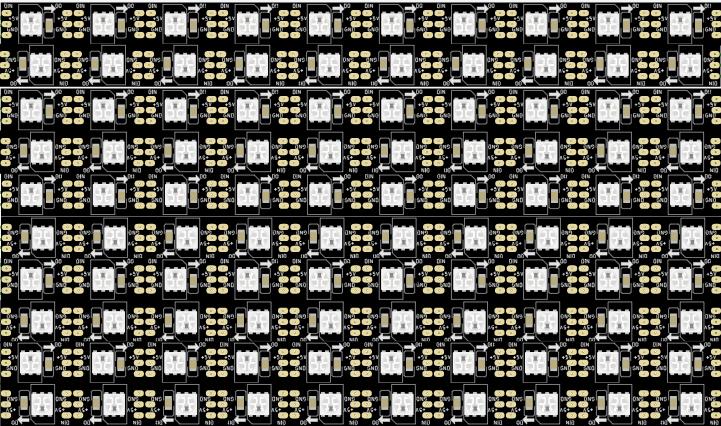
\includegraphics[width=4cm]{Matriz leds.png}
\centering
\caption{Matriz LEDs RGB}
\label{fig:Matriz leds.png}
\end{figure}


\end{document}
